\documentclass[12pt]{article}
\usepackage[utf8]{inputenc}
\usepackage{tgbonum}
\usepackage[a4paper, total={7in, 10in}]{geometry}
\usepackage{graphicx}
\usepackage{minted}
\title{Lab Assignment 8}
\author{Akshat Mittal - 20107}
\date{July 2021}
\begin{document}
\maketitle
\vspace{7mm}
\textbf{Contents}
\vspace{7mm}
\begin{enumerate}
    \item Creating and storing information in a file
    \item Reading and printing contents of file
    \item Writing multiple lines in text file
    \item Reversing string in a file word by word
    \item Displaying total and 4 letter words from a text file
    \item To merge two files
    \item Employee Management
    \item Size of a text file
    \item Displaying students record from a file sorted by their names
    \item Merging two files by alternate lines
    \item Counting lowercase, uppercase, digits, special characters in a file
    \item Writing student records in a file
    \item Student Management
\end{enumerate}

\newpage
\section{}
\subsection{Code}
\inputminted{c}{q1.c}
\subsection{Output}
\begin{figure}[h]
    \centering
    
\includegraphics[width=0.5\textwidth]{1.png}
\end{figure}
\subsection{Text File}
\inputminted{c}{q1.txt}

\newpage
\section{}
\subsection{Code}
\inputminted{c}{q2.c}
%\newpage
\subsection{Output}
\begin{figure}[h]
    \centering
    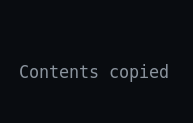
\includegraphics{2.png}
\end{figure}
\subsection{Text File}
\inputminted{c}{q2.txt}

\newpage
\section{}
\subsection{Code}
\inputminted{c}{q3.c}
\subsection{Output}
\begin{figure}[h]
    \centering
    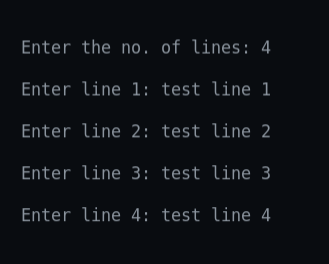
\includegraphics[width=0.5\textwidth]{3.png}
\end{figure}
\subsection{Text File}
\inputminted{c}{q3.txt}

\newpage
\section{}
\subsection{Code}
\inputminted{c}{q4.c}
\newpage
\subsection{Output}
\begin{figure}[h]
    \centering
    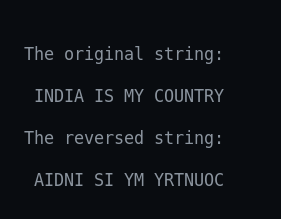
\includegraphics[width=0.8\textwidth]{4.png}
\end{figure}
\subsection{Text File}
\inputminted{c}{INPUT.TXT}

\newpage
\section{}
\subsection{Code}
\inputminted{c}{q5.c}
\newpage
\subsection{Output}
\begin{figure}[h]
    \centering
    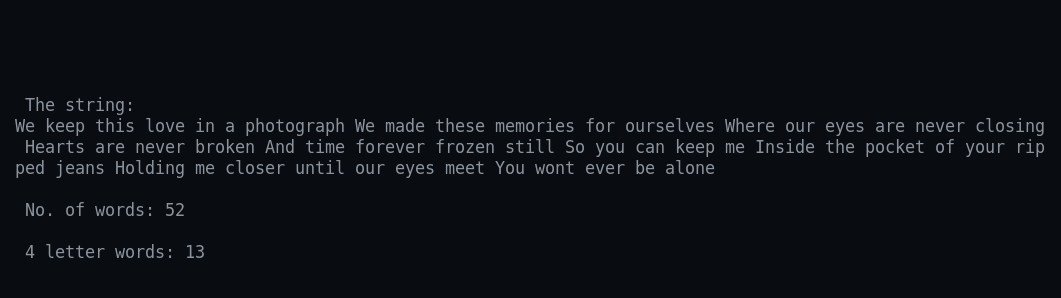
\includegraphics[width=1\textwidth]{5.png}
\end{figure}
\subsection{Text File}
\inputminted{c}{TRIAL.TXT}

\newpage
\section{}
\subsection{Code}
\inputminted{c}{q6.c}
\newpage
\subsection{Output}
\begin{figure}[h]
    \centering
    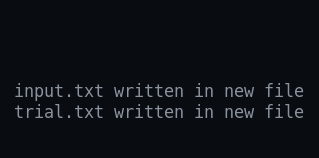
\includegraphics[width=0.8\textwidth]{6.png}
\end{figure}
\subsection{Text File}
\subsubsection{INPUT.TXT}
\inputminted{c}{INPUT.TXT}
\subsubsection{TRIAL.TXT}
\inputminted{c}{TRIAL.TXT}

\newpage
\section{}
\subsection{Code}
\inputminted{c}{q7.c}
\newpage
\subsection{Output}
\begin{figure}[h]
    \centering
    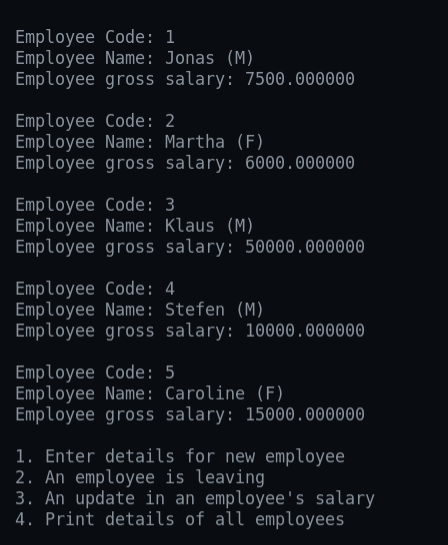
\includegraphics[width=0.8\textwidth]{7a.png}
\end{figure}
\newpage
\begin{figure}[h]
    \centering
    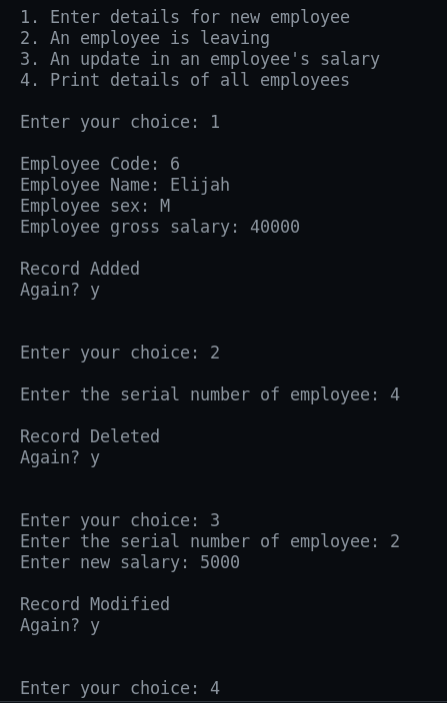
\includegraphics[width=0.7\textwidth]{7b.png}
\end{figure}
\newpage
\begin{figure}[h]
    \centering
    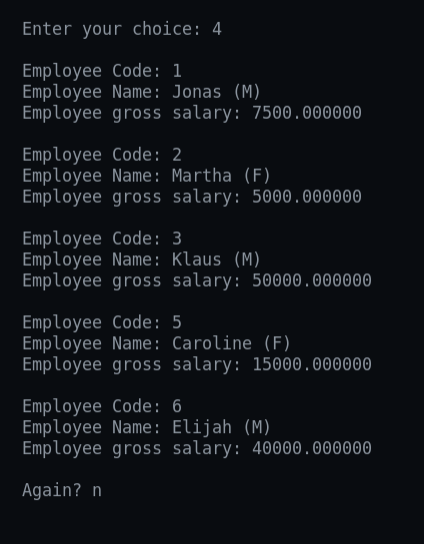
\includegraphics[width=0.8\textwidth]{7c.png}
\end{figure}

\newpage
\section{}
\subsection{Code}
\inputminted{c}{q8.c}
\subsection{Output}
\begin{figure}[h]
    \centering
    
\includegraphics[width=0.6\textwidth]{8.png}
\end{figure}
\subsection{Text File}
\inputminted{c}{TRIAL.TXT}
\newpage
\section{}
\subsection{Code}
\inputminted{c}{q9.c}
\newpage
\subsection{Output}
\begin{figure}[h]
    \centering
    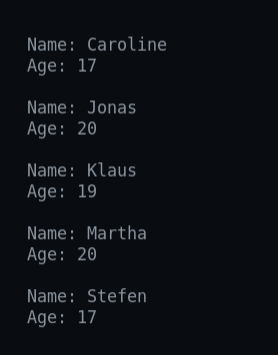
\includegraphics[width=0.75\textwidth]{9.png}
\end{figure}
\newpage
\section{}
\subsection{Code}
\inputminted{c}{q10.c}
\newpage
\subsection{Output}
\begin{figure}[h]
    \centering
    
\includegraphics[width=0.5\textwidth]{10.png}
\end{figure}
\subsection{Text File}
\subsubsection{q10a.txt}
\inputminted{c}{q10a.txt}
\subsubsection{q10b.txt}
\inputminted{c}{q10b.txt}
\subsubsection{q10.txt}
\inputminted{c}{q10.txt}

\newpage
\section{}
\subsection{Code}
\inputminted{c}{q11.c}
\newpage
\subsection{Output}
\begin{figure}[h]
    \centering
    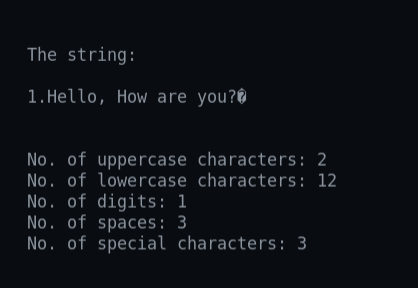
\includegraphics[width=0.75\textwidth]{11.png}
\end{figure}
\subsection{Text File}
\inputminted{c}{q11.txt}

\newpage
\section{}
\subsection{Code}
\inputminted{c}{q12.c}
\subsection{Output}
\begin{figure}[h]
    \centering
    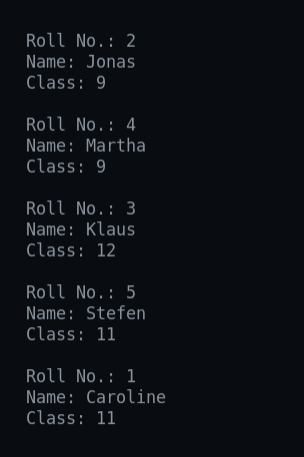
\includegraphics[width=0.6\textwidth]{12.png}
\end{figure}

\newpage
\section{}
\subsection{Code}
\inputminted{c}{q13.c}
\newpage
\subsection{Output}
\begin{figure}[h]
    \centering
    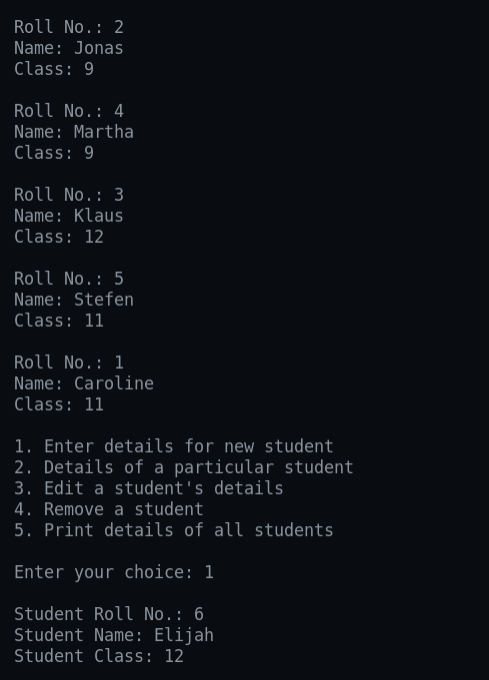
\includegraphics[width=0.8\textwidth]{13a.png}
\end{figure}
\newpage
\begin{figure}[h]
    \centering
    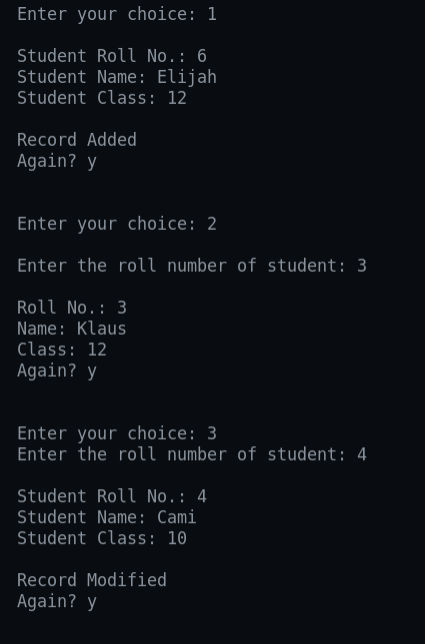
\includegraphics[width=0.8\textwidth]{13b.png}
\end{figure}
\newpage
\begin{figure}[h]
    \centering
    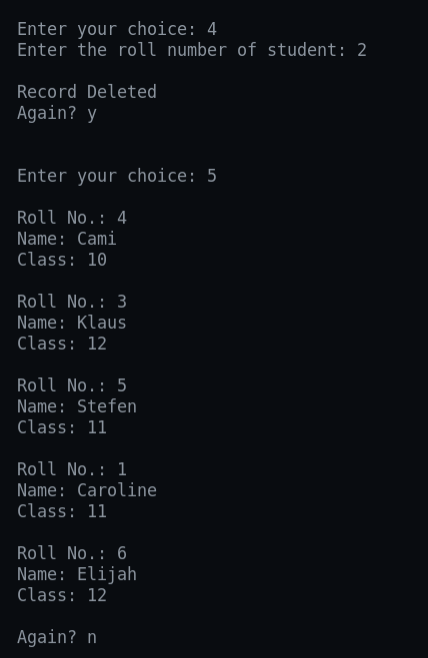
\includegraphics[width=0.8\textwidth]{13c.png}
\end{figure}
\end{document}